\documentclass[a4paper,titlepage]{report}
\usepackage{graphicx}
\usepackage[a4paper, margin=1in]{geometry}
\usepackage{titlesec}
\usepackage[dvipsnames]{xcolor}
\usepackage{amsmath}
\usepackage{booktabs}
\usepackage{cellspace}
\usepackage{tabularx}
\usepackage{caption}
\usepackage{calc}
\usepackage{ragged2e}
\usepackage{geometry}
\usepackage{multirow}

\setlength\cellspacetoplimit{5pt}
\setlength\cellspacebottomlimit{4pt}

\definecolor{myBlue}{rgb}{0.0745, 0.2157, 0.4118}
\definecolor{myLightBlue}{rgb}{0, 0.5647, 0.5843}

\titleformat{\section}[hang]{\Large\bfseries\color{myBlue}}{}{0px}{}[\titlerule]
\titleformat{\subsection}[hang]{\large\bfseries\color{myLightBlue}}{}{0em}{}
\titleformat{\subsubsection}[hang]{\bfseries\color{myBlue}}{}{0em}{}

% Set the dimension of titles of chapters to \LARGE and 
\titleformat{\chapter}[display]
  {\normalfont\Large\bfseries\color{myBlue}}{}{-80pt}{\LARGE}

% remove the word "Chapter" and the number from the title
\renewcommand{\chaptername}{}

\setcounter{tocdepth}{1} % Include only chapter and section in the table of contents

\begin{document}

\begin{titlepage}
    \centering
    \vspace*{\fill}
    {\LARGE \textbf{UNIVERSITY OF PISA}}\\[0.5cm]
    \begin{figure}[h]
        \centering
        
\includegraphics[width=0.5\textwidth]{images/universita-di-pisa-logo.png} 
    \end{figure}
    {\Large \textit{Artificial Intelligence and Data Engineering}}\\[1.5cm]
    {\LARGE \textbf{Distributed Systems and Middleware Technologies}}\\[1cm]
    {\Large \textit{FLconsole documentation}}\\[8cm]
    {\large \textbf{Authors: Çolak F. Messina F. Nocella F.}}\\[0.5cm]
    {\large Academic Year 2023/2024}
    \vspace*{\fill}
\end{titlepage}


\tableofcontents

\chapter{Introduction and Project Overview}

\section{Context and Project Objective}

The goal of this project is to develop a system to manage Federated Learning (FL) experiments. 
FL is a decentralized machine learning approach where multiple devices collaborate to train a 
shared model while keeping their data locally. The project aims to provide a graphic interface
 with a web console to run FL experiments, enabling users to monitor their progress and analyze 
 results. The system will use the Federated Learning Director (FL Director) to coordinate the 
 execution of experiments among the devices. The FL Director is an Erlang node that handle the 
 request of new experiments to propagate to the participants' devices. The system will be designed to support
  concurrent execution of multiple FL experiments, real-time analytics, and flexible storage
   of experiment statistics. The project will adopt the Model-View-Controller (MVC) pattern 
   to structure the Web Console, promoting separation of concerns and maintainability. The 
   system will utilize DocumentDB for flexible storage of experiment statistics and its
    horizontal scalability. Concurrent execution of experiments will be implemented using Java 
    threads and ExecutorService to optimize resource utilization. WebSocket communication 
    will be established for real-time data exchange, enabling seamless interaction between
     the frontend and backend. The project will define message formats and outline the structure
      of Erlang nodes for efficient communication. The system will provide a user-friendly
       Web Console to initiate and manage FL experiments, as well as centralized access to 
       experiment statistics for easy monitoring and analysis.

\section{Project Key Points}
\begin{itemize}
    \item Adopt the MVC (Model-View-Controller) pattern to structure the Web Console, promoting separation of concerns and maintainability.
    \item Utilize DocumentDB for flexible storage of experiment statistics and its horizontal scalability.
    \item Implement concurrent execution of experiments using Java threads and ExecutorService to optimize resource utilization.
    \item Establish WebSocket communication for real-time data exchange, enabling seamless interaction between the frontend and backend.
    \item Define message formats and outline the structure of Erlang nodes for efficient communication, ensuring reliability and scalability.
    \item System with a graphical interface and web console for executing FL experiments.
    \item Coordination of experiments through FL Director, an Erlang node.
    \item Real-time analytics and flexible storage of experiment statistics.
    \item Centralized access to experiment statistics for monitoring and analysis.
\end{itemize}

\chapter{Analysis}

\section{Requirements}

\subsection{Functional Requirements}

\subsubsection{For Administrators:}

\begin{itemize}
    \item Administrators must be able to log in to the application.
    \item Administrators must be able to log out of the application securely.
    \item Administrators must be able to create new configurations for experiments.
    \item Administrators must be able to create experiments based on the configurations they have defined.
    \item Administrators must be able to initiate experiments and oversee their execution.
    \item Administrators must be able to view other administrators' experiments.
    \item Administrators must possess the authority to perform CRUD operations on configurations and experiments.
    \item Administrators must be able to modify his/her own account information and delete account.
\end{itemize}

\subsubsection{For Users:}

\begin{itemize}
    \item Users must be able to log in to the application.
    \item Users must be able to log out of the application securely.
    \item Users must be able to register for a new account within the application.
    \item Users must be able to search for experiments based on configuration and experiment names.
    \item Users must be able to monitor real-time progress of experiments.
    \item Users must be able to modify his/her own account information and delete account.
\end{itemize}

\newpage
\subsection{Non-Functional Requirements}

\begin{enumerate}
    \item \textbf{Performance:} The system must handle a large number of concurrent users without significant performance degradation. Response times for critical operations should be kept within acceptable limits.
    \item \textbf{Reliability:} The system should be highly available with minimal downtime. 
    \item \textbf{Security:} User authentication and authorization mechanisms must be implemented.
    \item \textbf{Scalability:} The system should scale horizontally to accommodate increasing user loads and data volumes.
    \item \textbf{Usability:} The user interface must be intuitive and error messages must be informative.
    \item \textbf{Maintainability:} The codebase must be well-organized and documentation must be comprehensive.
    \item \textbf{Compatibility:} The application must be compatible with a wide range of web browsers and devices. Integration with external systems must be seamless.
\end{enumerate}

\section{Use Case Diagram}
\subsection{Actors}

The actors who can interact with the web console system consist of the following:
\begin{itemize}
    \item \textbf{User:} The user is the actor who can access to the system to browse all the experiments and view their progress.
    \item \textbf{Admin:} The admin is the actor who can manage the system, including creation and deletion of configurations and experiments, running the experiments and view their progress.
\end{itemize}

\begin{figure}[ht!]
    \centering
    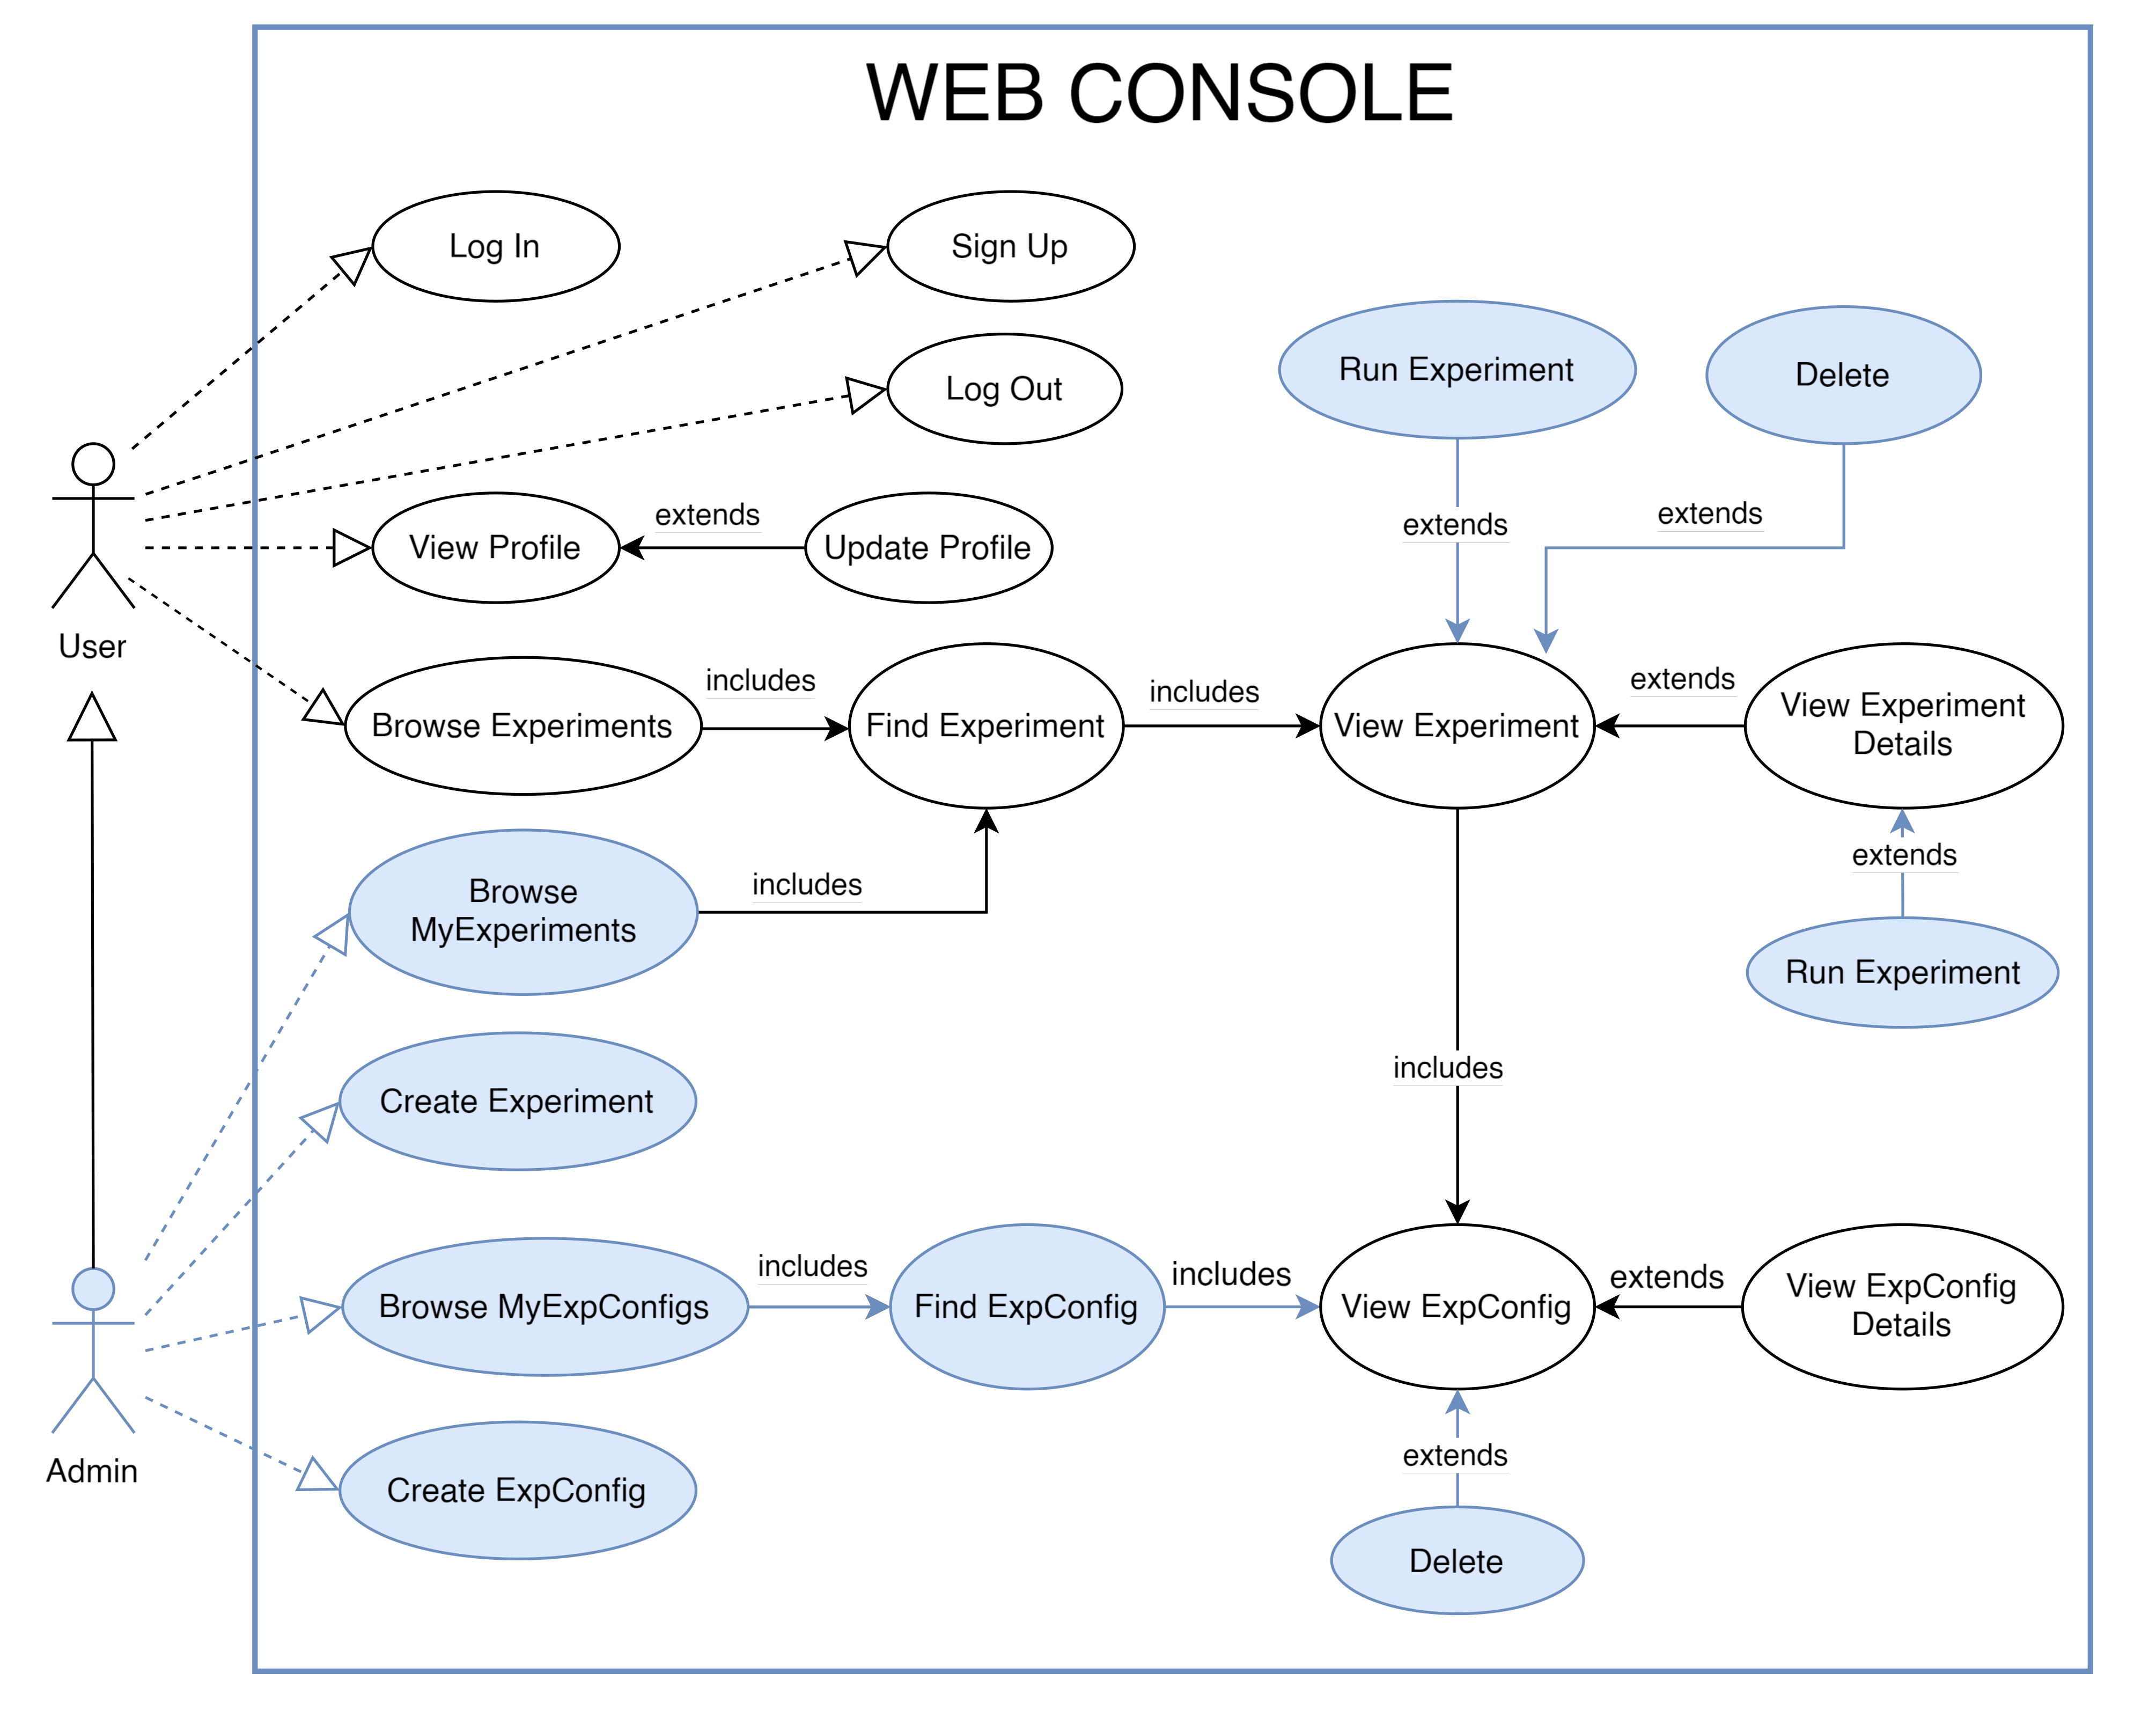
\includegraphics[width=0.8\textwidth]{images/2_analisys/FL_use_case.png}
    \caption{Use Case Diagram}
    \label{fig:use_case_diagram}
\end{figure}

\newpage
\subsection{Scenarios}
In the following tables, several key use cases related to the management and execution of experiments within the application are presented. These use cases cover actions performed by different actors, including users and administrators, and describe the steps involved in each scenario, along with pre-conditions and post-conditions.
\begin{table}[ht!]
    \centering
    \caption{Use Case: Find Experiment}
    \begin{tabularx}{\textwidth}{|Sl|S{X}|}
        \hline
        \textbf{\textit{Use Case}}       & \textbf{Find Experiment}                                           \\ \hline
        \textbf{Primary Actor}           & User, Admin                                                        \\ \hline
        \textbf{Secondary Actor}         & --                                                                 \\ \hline
        \textbf{Description}             & Allows the actor to find a specific experiment                     \\ \hline
        \textbf{Pre-Conditions}          & Actor must be logged in                                            \\ \hline
        \textbf{Main event steps}        & 1. The actor navigates to the “Search” feature                     \\
                                         & 2. The actor enters the Experiment and/or the configuration name   \\
                                         & 3. The system searches for the list of experiments in database for \\
                                         & matching results                                                   \\ \hline
        \textbf{Post-Conditions}         & The actor views a list of experiments matching the                 \\
                                         & search criteria if there are any                                   \\ \hline
        \textbf{Correlated Use cases}    &                                                                    \\ \hline
        \textbf{Alternative event steps} & --                                                                 \\ \hline
    \end{tabularx}
\end{table}

\begin{table}[ht!]
    \centering
    \caption{Use Case: Create Experiment}
    \begin{tabularx}{\textwidth}{|Sl|S{X}|}
        \hline
        \textbf{\textit{Use Case}}       & \textbf{Create Experiment}                                        \\ \hline
        \textbf{Primary Actor}           & Admin                                                             \\ \hline
        \textbf{Secondary Actor}         & --                                                                \\ \hline
        \textbf{Description}             & Allows the admin to create a specific experiment                  \\ \hline
        \textbf{Pre-Conditions}          & Actor must be logged in and has the admin privileges              \\ \hline
        \textbf{Main event steps}        & 1. Admin selects the option to create a new experiment.           \\
                                         & 2. Admin fills in the name and configurations for the experiment. \\
                                         & 3. Admin confirms the creation of the experiment.                 \\ \hline
        \textbf{Post-Conditions}         & The experiment is successfully created.                           \\ \hline
        \textbf{Correlated Use cases}    & Run Experiment                                                    \\ \hline
        \textbf{Alternative event steps} & --                                                                \\ \hline
    \end{tabularx}
\end{table}



\begin{table}[ht!]
    \centering
    \caption{Use Case: Run Experiment}
    \begin{tabularx}{\textwidth}{|Sl|S{X}|}
        \hline
        \textbf{\textit{Use Case}}       & \textbf{Run Experiment}                                                     \\ \hline
        \textbf{Primary Actor}           & Admin                                                                       \\ \hline
        \textbf{Secondary Actor}         & --                                                                          \\ \hline
        \textbf{Description}             & Allows the admin to start a specific experiment                             \\ \hline
        \textbf{Pre-Conditions}          & Actor must be logged in and have admin privileges                           \\ \hline
        \textbf{Main event steps}        & 1. Admin selects the experiment and reaches the details page.               \\
                                         & 2. If the experiment has not started yet                                         \\
                                         & \hspace{1em} 2.1 When the start button is clicked \\
                                         & \hspace{2.5em} 2.2 The system will send a request to start the experiment \\
                                         & \hspace{2.5em} 2.3 If the experiment is successfully started, the system will \\
                                         & \hspace{2.5em} display a success message \\ \hline
        \textbf{Post-Conditions}         & The experiment statistics are shown on the experiment details page          \\
                                         & and saved in the database.                                                  \\ \hline
        \textbf{Correlated Use cases}    &                                                                             \\ \hline
        \textbf{Alternative event steps} & --                                                                          \\ \hline
    \end{tabularx}
\end{table}

\begin{table}[ht!]
    \centering
    \caption{Use Case: View Experiment Progress}
    \begin{tabularx}{\textwidth}{|Sl|S{X}|}
        \hline
        \textbf{\textit{Use Case}}       & \textbf{View Experiment Progress}                                                     \\ \hline
        \textbf{Primary Actor}           & User, Admin                                                        \\ \hline
        \textbf{Secondary Actor}         & --                                                                          \\ \hline
        \textbf{Description}             & Allows the admin to view a specific experiment progress                            \\ \hline
        \textbf{Pre-Conditions}          & Actor must be logged in and have admin privileges                           \\ \hline
        \textbf{Main event steps}        & 1. The actor selects the experiment and reaches the details page.               \\
                                        & 2. If the experiment is started                                        \\
                                        & \hspace{1em} 2.1 Retrieve the stored progresses from the database \\
                                        & \hspace{1em} 2.2 Display the progress on the experiment details page\\
                                        & 3. If the experiment is running                    \\
                                        & \hspace{1em} 3.1 Connect to the websocket\\
                                        & \hspace{1em} 3.2 Subscribe to the experiment progress topic\\
                                        & \hspace{1em} 3.3 While the experiment is running, display the progress in  \\
                                        & \hspace{1em} real-time each time a new message is received\\
                                        & \hspace{1em} 3.4 Unsubscribe from the topic and disconnect from websocket \\ 
                                        & \hspace{1em} when the experiment is finished\\ \hline
        \textbf{Post-Conditions}       & The experiment progress is displayed on the experiment details page.          \\ \hline
        \textbf{Correlated Use cases}    &                                                                             \\ \hline
        \textbf{Alternative event steps} & --                                                                          \\ \hline
    \end{tabularx}
\end{table}

\newpage
\section{Analysis Class Diagram}

\begin{figure}[ht!]
    \centering
    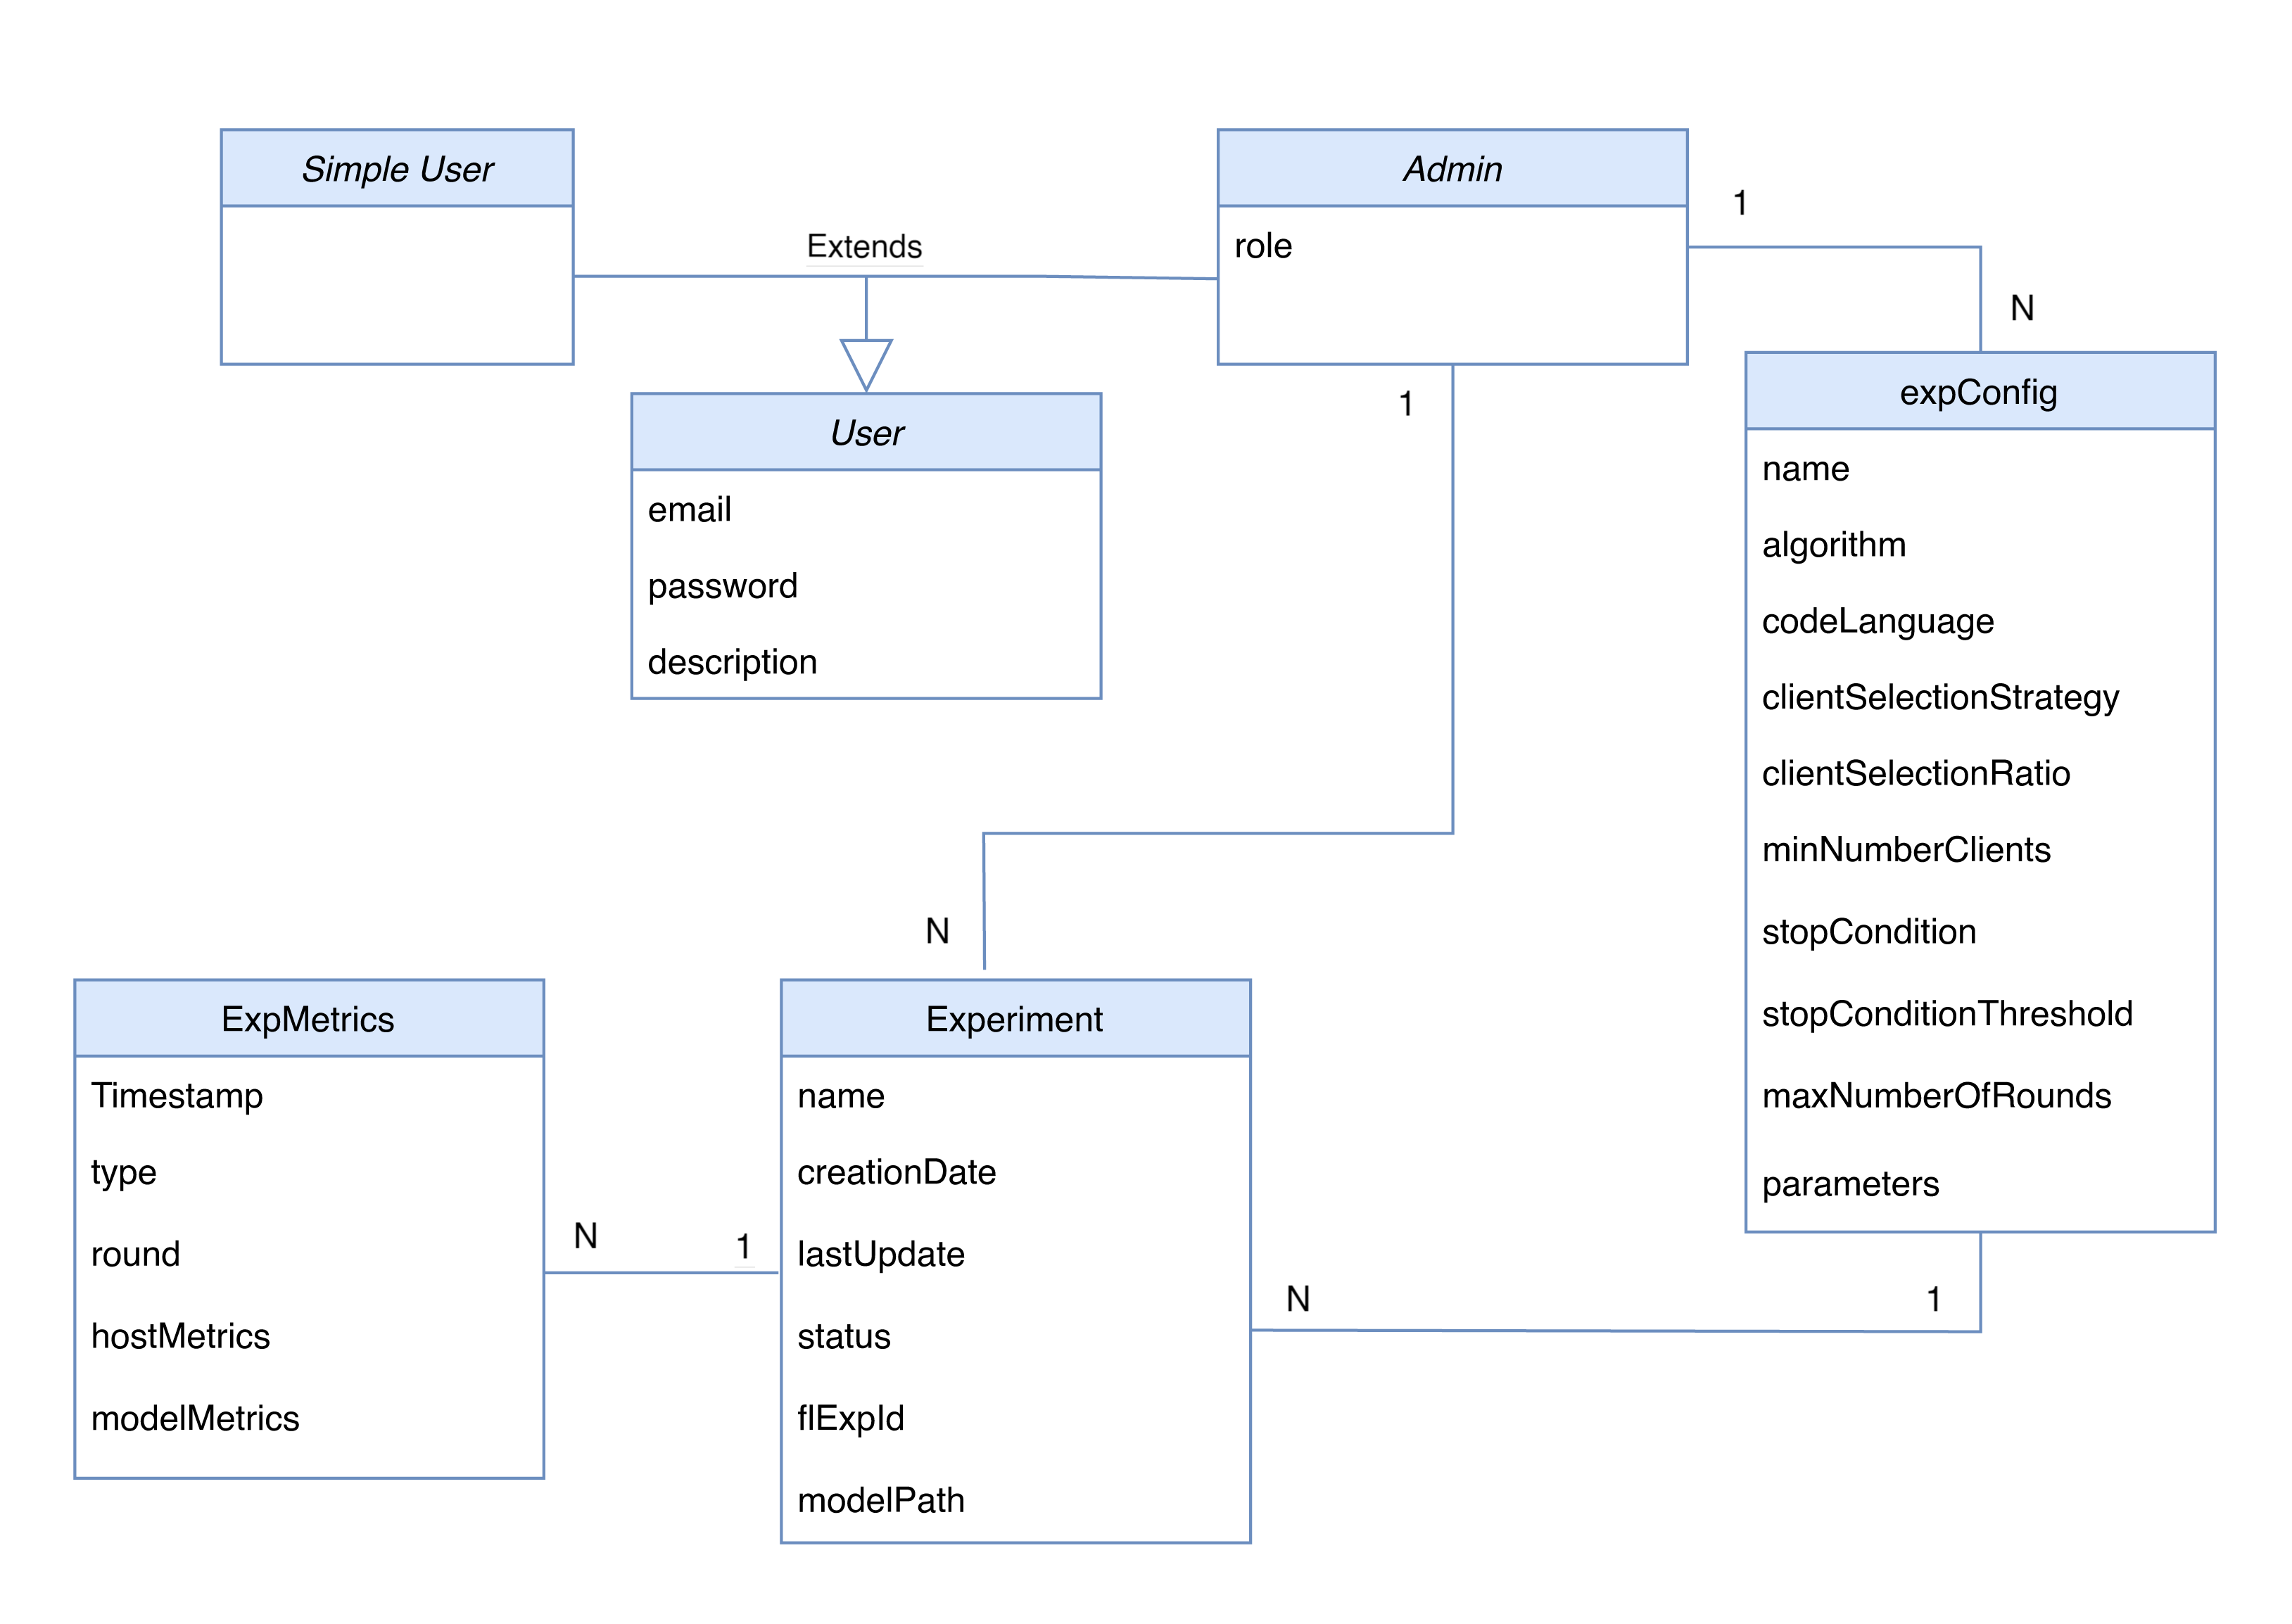
\includegraphics[width=0.9\textwidth]{images/2_analisys/FL_class_diag.png}
    \caption{Class Diagram}
    \label{fig:class_diagram}
\end{figure}

\newpage
\section{Sequence Diagrams}
The following sequence diagrams illustrate the interactions between the actors and the system for the key use
cases described in the previous section: the request to start an experiment and the request to view the progress
of an experiment.
\begin{figure}[ht!]
    \centering
    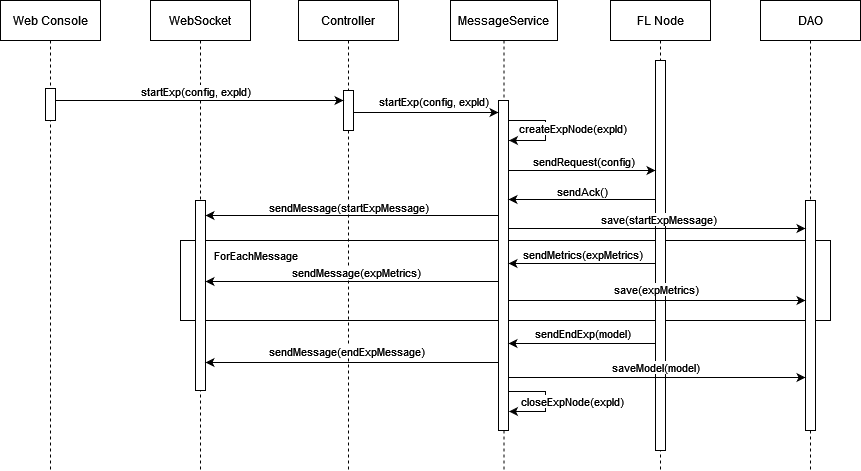
\includegraphics[width=0.9\textwidth]{images/2_analisys/sequence-diagram-start-exp.png}
    \caption{Sequence Diagram - Start Experiment}
    \label{fig:sequence_diagram_start_exp}
\end{figure}

\begin{figure}[ht!]
    \centering
    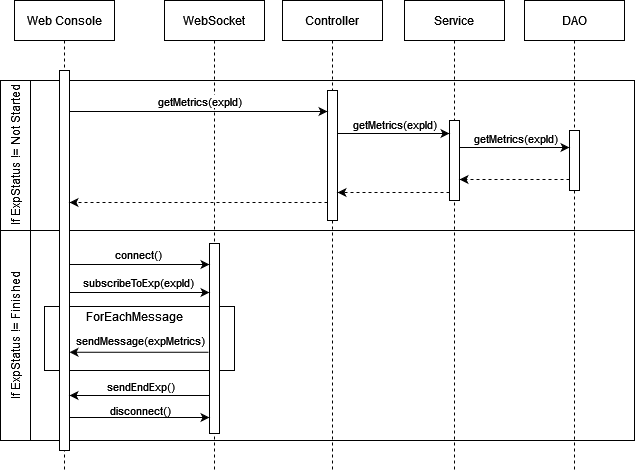
\includegraphics[width=0.9\textwidth]{images/2_analisys/sequence-diagram-view-progress.png}
    \caption{Sequence Diagram - View Progress}
    \label{fig:sequence_diagram_view_progress}
\end{figure}



\chapter{Design}

\section{Introduction}
This chapter aims to provide a detailed overview of the software architecture and database design of the project. It is essential for understanding the organization and structure of the system, as well as the design choices made to ensure the efficiency, scalability, and robustness of the software.

The design of the software architecture focuses on the organization and distribution of software components, defining roles, responsibilities, and interactions among them. Key architectural decisions guiding the project's development will be presented within this context.

Additionally, the database design will be examined, with particular attention to the decision to use a NoSQL database like MongoDB. This decision was motivated by the need to adapt to the specific requirements of the project, including flexible management of unstructured data and horizontal scalability.


\section{Software Architecture}

\begin{figure}[ht!]
    \centering
    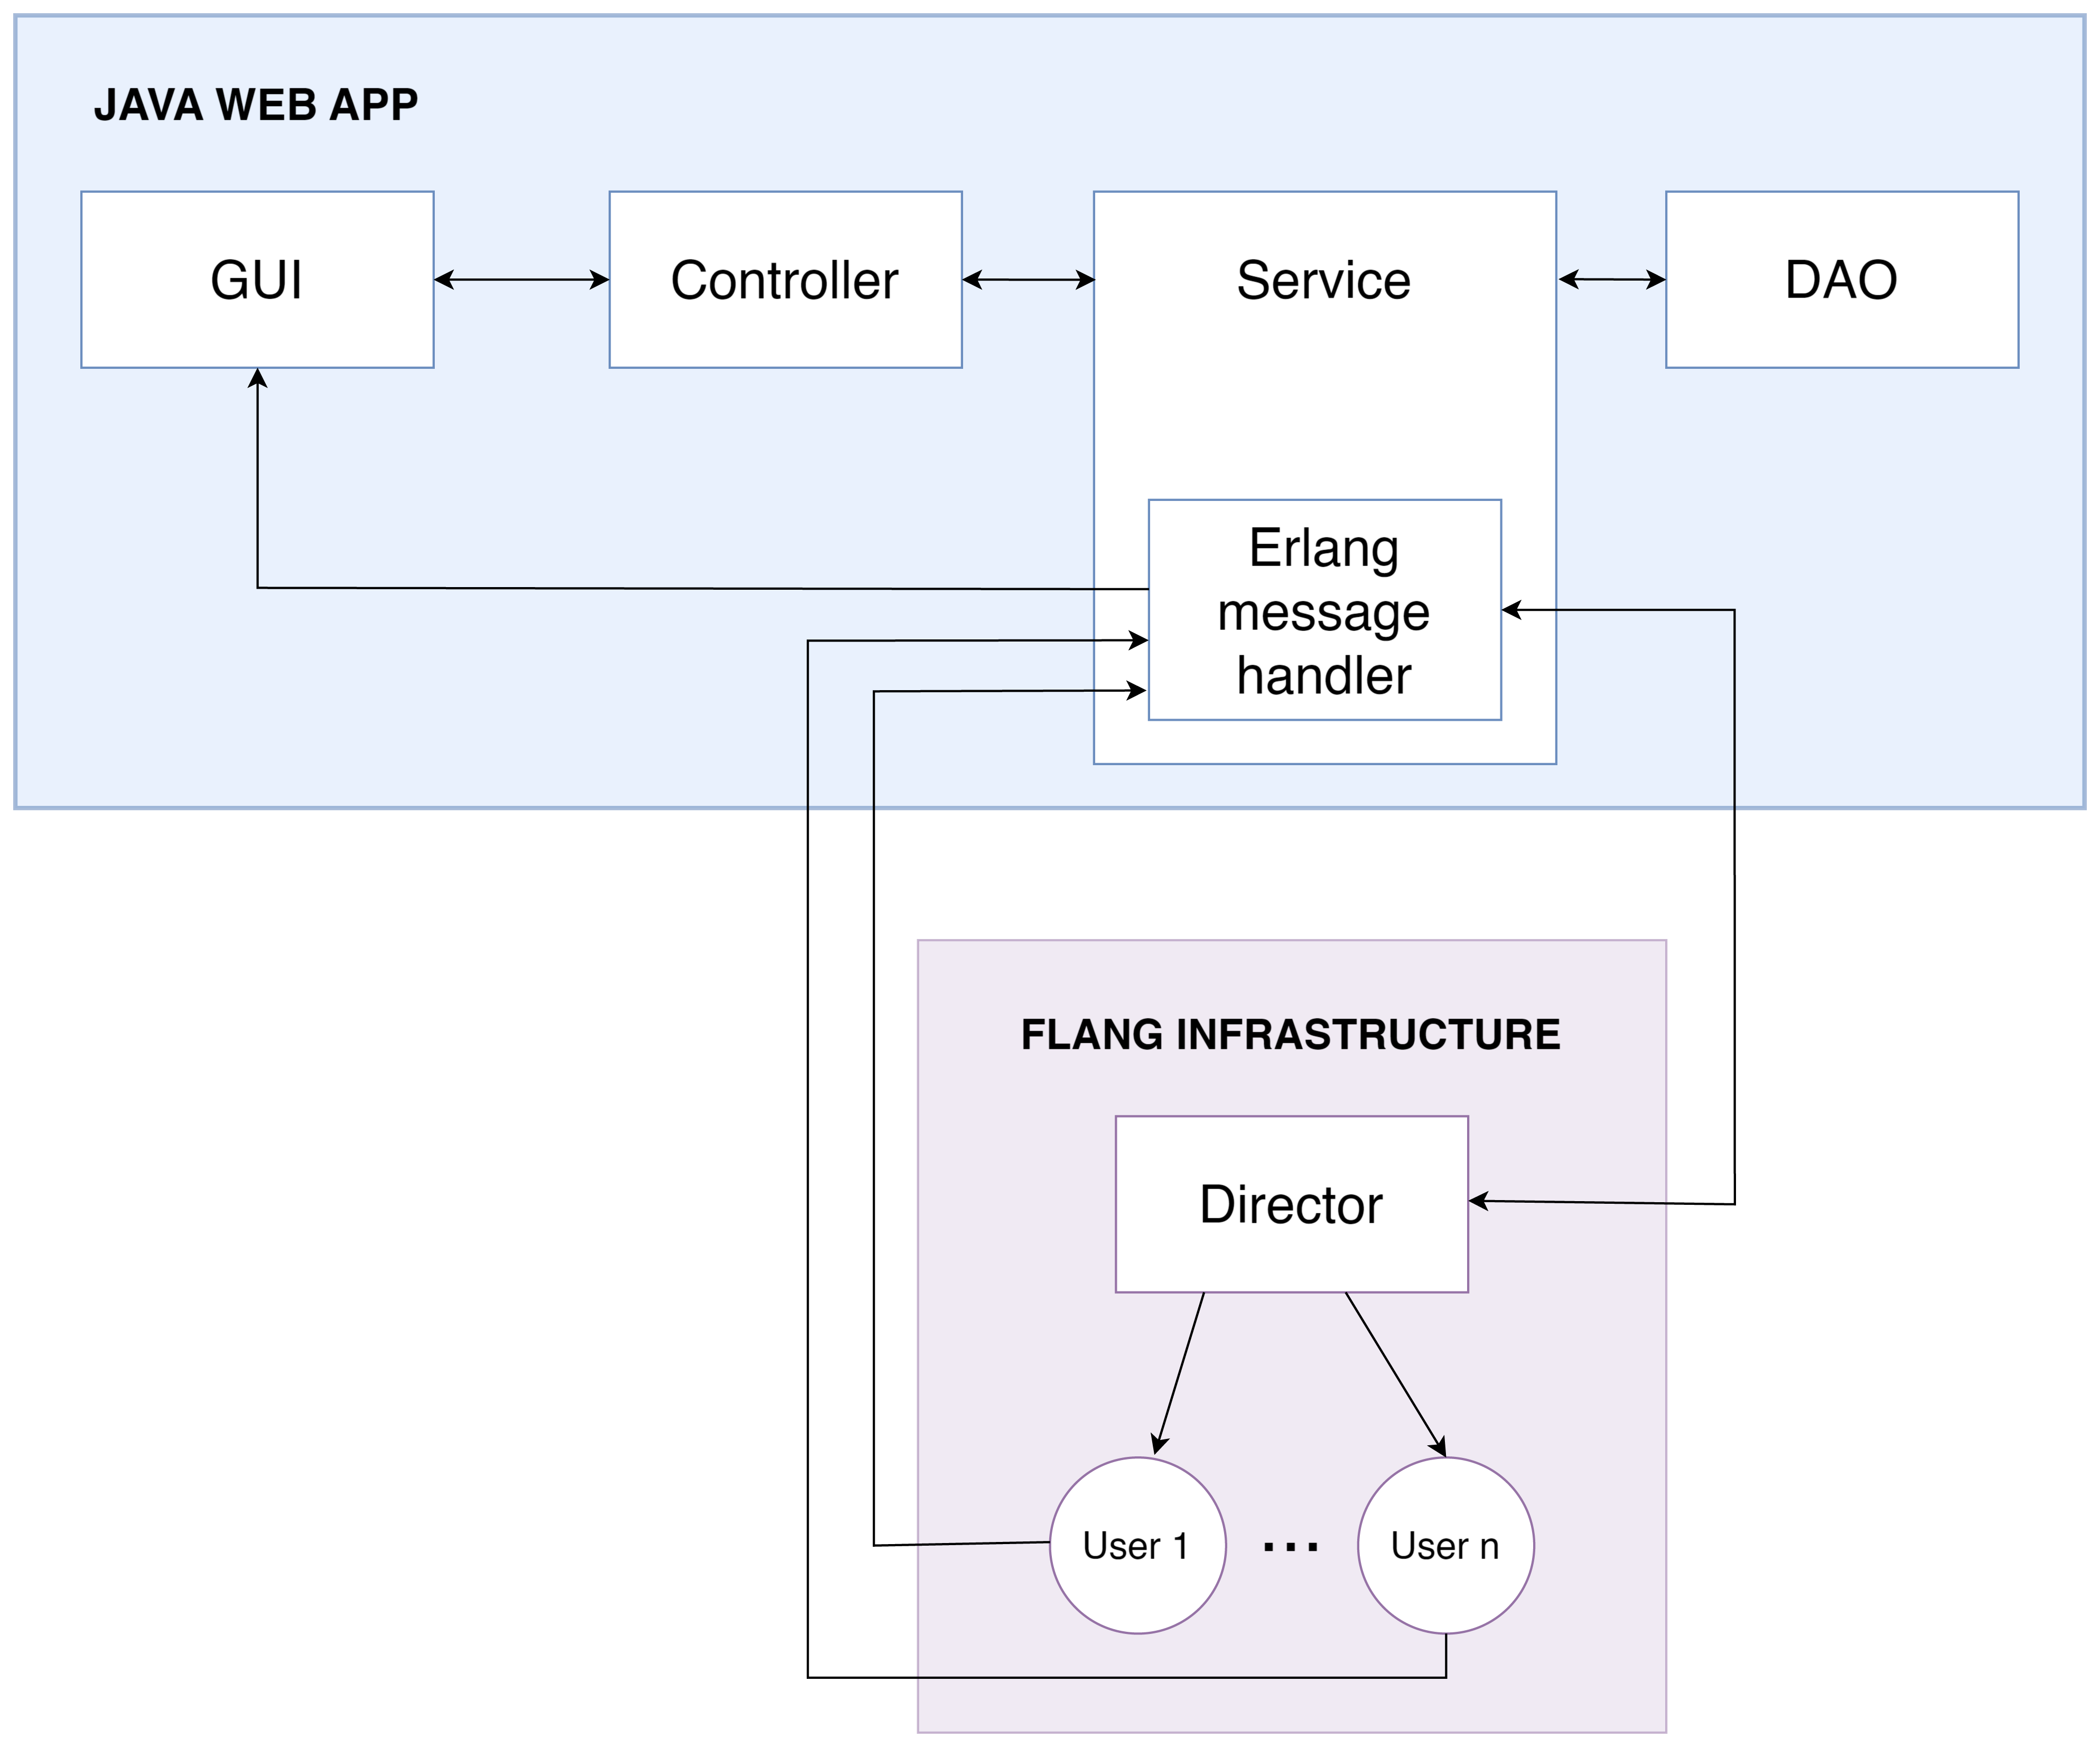
\includegraphics[width=0.8\textwidth]{images/2_analisys/FL_proj_Arch_FINAL.png}
    \caption{System Architecture}
    \label{fig:system_architecture}
\end{figure}


\newpage
\section{Database Design}

\subsection{MongoDB}
\subsubsection{Collections}
\textbf{ExpConfig document example:} \begin{verbatim}
        {
            "_id": {
              "$oid": "6613f8b7aed2e52b006dea10"
            },
            "name": "TestConfig",
            "algorithm": "fcmeans",
            "codeLanguage": "python",
            "clientSelectionStrategy": "probability",
            "clientSelectionRatio": 1,
            "minNumberClients": 2,
            "stopCondition": "max_number_rounds",
            "stopConditionThreshold": 5,
            "maxNumberOfRounds": 10,
            "parameters": {
              "targetFeature": "16",
              "lambdaFactor": "2",
              "numFeatures": "16",
              "seed": "10",
              "numClusters": "10"
            },
            "creationDate": {
              "$date": "2024-04-08T14:01:27.232Z"
            },
          }
    \end{verbatim}
\textbf{Experiment document example:} \begin{verbatim}
        {
            "_id": {
              "$oid": "661c3d780bb4be3bd9b891b9"
            },
            "name": "ExpTest",
            "expConfig": {
              "_id": {
                "$oid": "6613f8b7aed2e52b006dea10"
              },
              "name": "TestConfig",
              "algorithm": "fcmeans"
            },
            "creationDate": {
              "$date": "2024-04-14T20:32:56.022Z"
            },
            "status": "FINISHED",
            "flExpId": "\"d9d1bc7c-d733-4219-b4fb-16a3849db323\"",
            "modelPath": "\\FL_models\\exp_661c3d780bb4be3bd9b891b9.bin"
          }

    \end{verbatim}

\newpage
\textbf{ExperimentMetrics document example:} \begin{verbatim}
        {
            "_id": {
              "$oid": "66144b5337a2fd7f67582f67"
            },
            "expId": "661c3d780bb4be3bd9b891b9",
            "type": "STRATEGY_SERVER_METRICS",
            "hostMetrics": {
              "cpuUsagePercentage": 5,
              "memoryUsagePercentage": 9.27
            },
            "modelMetrics": {
              "FRO": 845.7339394664009
            },
            "timestamp": {
              "$date": "1970-01-20T19:43:26.034Z"
            },
            "round": 1,
          }
    \end{verbatim}

\textbf{User document example:} \begin{verbatim}
    {
        "_id": {
          "$oid": "6611252030f96a50aebda458"
        },
        "email": "admin@example.com",
        "password": "P@ssw0rd",
        "description": "example description of a user",
        "creationDate": {
          "$date": "2024-04-06T10:34:08.669Z"
        },
        "role": "admin",
        "configurations": [
          "6613f8b7aed2e52b006dea10"
        ],
        "experiments": [{
            "_id": {
              "$oid": "661c3e800bb4be3bd9b891da"
            },
            "name": "ExpTest",
            "config": "TestConfig",
            "creationDate": {
              "$date": "2024-04-14T20:32:56.022Z"
            }
          }]
      }

    \end{verbatim}
\newpage
\section{Message Handler}

\subsection{JInterface for Message Passing}
The message handler is implemented using the Erlang programming language. Erlang is a functional
programming language designed for building scalable and fault-tolerant systems. It is
particularly well-suited for building distributed systems, thanks to its lightweight
processes and built-in support for message passing. In this project, it's utilized the 
JInterface library, which allows to write Java code that can communicate with Erlang 
processes to send and receive messages. Rather than using directly Erlang nodes with Erlang language and communicate with them
through web socket, the choice of adopting JInterface library provides manipulation of messages directly in 
Java, storing the information contained in the messages in database and sending them to frontend.

\subsection{Message Structure}
Almost all the messages sent from the FLang Infrastructure to the Erlang message handler are tuples containing one atom to specify the
message type and a string for the message body in Json format. The json string contains the information about the message, such as the timestamp,
the round number, the client id, and the metrics. The following are some examples of message bodies in json format:
\begin{itemize}
    \item Experiment Queued:
    \begin{verbatim}
        {
            "type": "experiment_queued",
            "timestamp": "1712206255"
        }
    \end{verbatim}

    \item Worker Ready:
    \begin{verbatim}
        {
            "type": "worker_ready",
            "timestamp": "1712206257",
            "client_id": "1"
        }
    \end{verbatim}

    \item Strategy Server Ready:
    \begin{verbatim}
        {
            "type": "strategy_server_ready",
            "timestamp": "1712206257"
        }
    \end{verbatim}

    \item All Workers Ready:
    \begin{verbatim}
        {
            "type": "all_workers_ready",
            "timestamp": "1712206257"
        }
    \end{verbatim}

    \item Start Round:
    \begin{verbatim}
      {
          "type": "start_round",
          "timestamp": "1712206257",
          "round": "1"
      }
    \end{verbatim}

    \newpage

    \item Woker Metrics:
    \begin{verbatim}
      {
        "type": "woker_metrics",
        "timestamp": "1712206258",
        "round": "1"
        "client_id": "1"
        "hostMetrics": {
          "cpuUsagePercentage":39.4,
          "memoryUsagePercentage": 52.69
        }
        "modelMetrics":{
          "ARI":"0.10764575464353877"
        }
      }
    \end{verbatim}

    \item End Round:
    \begin{verbatim}
      {
        "type": "end_round",
        "timestamp": "1712206260",
        "round": "1"
      }
    \end{verbatim}

    \item Strategy Server Metrics:
    \begin{verbatim}
      {
        "type": "strategy_server_metrics",
        "timestamp": "1712206264",
        "round": "2",
        "hostMetrics": {
          "cpuUsagePercentage":39.4,
          "memoryUsagePercentage": 52.69
        }
         "modelMetrics":{
          "FRO":"0.13237183370436725"
        }
      }
    \end{verbatim}
   
\end{itemize}

\subsection{}
The trained model is sent at the end of the experiment in a special message that consists of a tuple with arity 3, \
where the first element is the message type's atom ``fl\_end\_str\_run'',
the second element is the identifier used by the FLang Infrastructure to identify the experiment, and the third element is the model in binary format.
\\
The message structure is designed to be flexible and extensible, allowing for easy integration of new message types and
additional information as needed. This design choice enables the system to adapt to changing requirements and accommodate
future enhancements without significant modifications to the existing codebase.

\subsection{Description of the Erlang Message Handler Module}
The Erlang message handler module is a crucial component of the system responsible for managing incoming messages, processing them accordingly, and facilitating communication between different parts of the distributed system. It encapsulates the logic for handling various types of messages, such as error notifications, stop signals, and data updates, ensuring proper routing and processing. Additionally, the module provides interfaces for sending and receiving messages, abstracting the underlying communication mechanisms and enabling seamless integration with other system components. Its robust design and fault-tolerant features contribute to the overall reliability and performance of the distributed system.
\chapter{Implementation}

\section{Development Environment}

%The development environment used for the project is described in this section.
To be able to have efficient and successful implementation of Federated Learning Web Console Project, having a well-chosen development environment is one of the
most important aspects. In this section, it is specified that the necessary tools, frameworks, and configuration requirements of the project. \\
\begin{itemize}
    \item \textbf{Programming Language:} Java is used for creating a Web Application. Erlang is used for facilitation the development of middleware component and FL director is an Erlang node.
          So that effective communication between the Web Application and the FL director is provided.
    \item \textbf{Frameworks:} Spring is used for Java framework. It ensures to integrate dependencies for WebSocket communication and MongoDB support.
          WebSocket is implemented to provide real-time communication between frontend and backend components.
    \item \textbf{Database Management:} MongoDB is chosen as a database to ensure storing data for experiment statistics and user information.
    \item \textbf{Version Control:} Git is used for version control. It is used to manage the source code of the project. GitHub is used to provide a collaborative development with its version control system. Efficient code management and collaboration is ensured by using repositories which is provided by the platform itself.
    \item \textbf{Integrated Development Environment:} IntelliJ IDEA is used as an IDE. It is a Java integrated development environment for developing computer software. It is developed by JetBrains. It is used to write, compile, and run the code. It also provides a user-friendly interface for developers.
    \item \textbf{Build Automation:} Maven is used for build automation. It is a build automation tool used primarily for Java projects. It is used to manage the project's build, reporting, and documentation from a central piece of information. Maven is used to control project dependencies and build configurations.
    \item \textbf{Testing: } Junit testing is used for testing Java code.
\end{itemize}


\section{Main Modules}

%The main modules of the project are described in this section.
Implementation of the project is structured by diving the project into modules. Each module ensures specific requirements of the project architecture. The modules are:\\
\begin{itemize}
    \item Configuration
    \item Controller
    \item DAO (Data Access Object)
    \item DTO (Data Transfer Object)
    \item Model
    \item Service
    \item Utils
\end{itemize}

\section{Configuration}

%The configuration of the project is described in this section.
Configuration classes of the Federated Learning Web Console project are created to provide responsibilities for configuring different parts of the application such as
logging, execution, HTTP request handling, MVC setup and WebSocket communication. Efficient operation, security and scalability of the system can be ensured by those configuration properties.

\section{Data Access}

%The data access layer of the project is described in this section.
The data access classes are fulfilling the requirements of interacting with the database layers, providing data retrieval, storage, and manipulation. This module includes classes with CRUD
(create, read, update, delete) operations and query executions. With the Data Access classes such as ExpConfigDao, ExperimentDao, MetricsDao, UserDao the application guarantees effective operations,
management of experiments and tracking of the progress.


\section{Data Transfer}

%The data transfer mechanisms used in the project are described in this section.
Data Transfer layer contains a ExpConfigSummary, ExperimentSummary and UserSummary classes to ensure the functionality of transferring data structure between different layers and components of the application. With the help of the DTO classes,
related information will be able to be transferred between frontend, backend, and service layers. User information is transferred in a more standardized way
for achieving better communication.

\section{Service}

%The services provided by the project are described in this section.
Service module includes business logic and operations for ensuring the fully functional application. It provides data processing and interaction between different components. Service module includes:\\
\begin{itemize}
    \item Cookie Service is for managing cookie operations such as cookie creation, retrieval, and deletion. The purpose of this service is ensuring session management and personalized user experience.
    \item Experiment Configuration Service is for implementing business logic for experiment configuration includes creation, deletion, retrieval and searching by some parameters.
    \item Experiment Service is for creating operations that are related with experiment like creation, running, deletion, retrieval and searching.
    \item User Service is implemented for ensuring business logic for user-based operations. Those operations include authentication of user, sign up, deletion of account, updating user information and retrieval of the user
    \item Message Service is implemented for managing communication with Erlang node for sending experiment configuration and monitoring the progress.
    \item Metrics Service is created to handle operations of retrieving experiment metrics from the database with the related experiment ID.
\end{itemize}

\section{Controller}

The Controller module within our MVC pattern web application encompasses two primary classes: the Main
Controller and the Admin Controller. These classes serve as the intermediaries between the user's requests 
and the application's backend logic. Their main function is to interpret user requests, process any input 
parameters provided, and then direct the flow of control accordingly, often rendering dynamic content 
onto static pages for the user to interact with.

\section{Utils}

The Utils module serves as a foundational component within our application, housing a collection of 
classes that provide essential functionality utilized across our Java codebase. These classes encompass 
a wide range of utilities, including enumerations, exception handling, email and password validation 
mechanisms, and the management of constants and cryptographic operations.

\section{User Interface}

%The user interface of the project is described in this section.
User Interface module is responsible for providing a user-friendly interface for the users. This module makes application functionalities visible for the end-user. It includes the following components:\\
\begin{itemize}
    \item Login and Sign Up Page: This page is for user authentication and registration. Users can log in to the system by providing their email and password. If the user does not have an account, they can sign up by providing their email, password, and description.
    \item User Dashboard: This page is for displaying the experiments to the user. Users can see experiments and their progress on this page.
    \item Experiment Page: This page is for displaying the details of the experiment. The page shows the details of the experiment and its progress on this page.
    \item Admin Dashboard: This page is for displaying all experiments and admin's own configurations. Admins can see all experiments and their progress on this page and also it provides creating and deleting experiments and configurations for the admin.
    \item Profile Page: The profile page allows users to view and manage their account settings and profile information.
\end{itemize}

\section{Adopted Patterns and Techniques}

%The patterns and techniques adopted in the project are described in this section.

During the implementation of the Federated Learning Web Console project, various patterns and techniques are adopted to ensure the efficiency, scalability, and maintainability of the application. These are some of the used patterns and techniques:\\

\subsection{Model-View-Controller (MVC) Pattern}
The Federated Learning Web Console project is implemented by following the Model-View-Controller (MVC) pattern. This pattern is used to separate the application into three main components: Model, View, and Controller. The Model represents the data and business logic
of the application, the View represents the presentation layer, and the Controller handles the user input and updates the model and view accordingly. This pattern ensures a clean separation of concerns and makes the application easier to maintain and extend.\\

\subsection{WebSocket Communication}
WebSocket communication is implemented to provide real-time communication between the frontend and backend. This allows the application to send and receive messages in real-time without the need for polling or long-polling. WebSocket communication is used to update the user interface with the latest data and provide a seamless user experience.\\

\subsection{Asynchronous Processing}
Asynchronous processing techniques like Java threads and ExecutorService are e used to manage concurrent execution of experiments. This allows the application to handle multiple requests and tasks simultaneously and improve performance and scalability.\\

\subsection{Message Passing Protocol}
To achieve seamless communication between Erlang FL director and Java web application, a customized and well specified message passing protocol is defined. This protocol guarantees the reliable and well-defined exchange of messages and data.


% \section{System configuration}
% \subsection{MongoDB}
% Per ogni replica che si vuole aggiungere al replica set è necessario avviare un'istanza di MongoDB con il comando:
% mongod --replSet SETNAME --dbpath PATH --port PORT --bind_ip localhost,IP --oplogSize 200

% nel nostro caso è stato fatto con tutti i cluster forniti.
% mongod --replSet DSMT --dbpath ~/data --port 27017 --bind_ip localhost,10.2.1.109 --oplogSize 200

% una volta che i cluster sono tutti online bisogna connettersi al primary, nel nostro caso

% mongosh --host 10.2.1.109 --port 27017

% fornire la configurazione
% rsconf = {_id: "dsmt", members: [{_id: 0, host: "10.2.1.103", priority:1},{_id: 1, host: "10.2.1.106", priority:2},{_id: 3, host: "10.2.1.107", priority:3},{_id: 4, host: "10.2.1.108", priority:4},{_id: 2, host: "10.2.1.109", priority:5}]};

% e inizializzare il replica set con il comando

% rs.initiate()

% Dopo ciò le repliche saranno operative e sarà possibile connettersi.

% \subsection{Tomcat}
% La prima cosa da fare è copiare il file .war all'interno della cartella webapps di Tomcat. per farlo abbiamo usato scp
% scp MY_LOCAL_PATH root@REMOTE_IP:/REMOTE_PATH/apache-tomcat-10.1.16/webapps/FILENAME.war

% Per avviare il server Tomcat è necessario entrare nel path dove è installato ed eseguire il comando:

% bin/startup.sh

% nel nostro caso :
% ./servers/apache-tomcat-10.1.16/bin/startup.sh

% \subsection{Nginx}
% Una volta scaricato Nginx è necessario configurare il file di configurazione per farlo abbiamo usato nano
% nano /etc/nginx/nginx.conf

% aggiungendo

% server {
% listen 80;
% server_name 10.2.1.102;  # IP pubblico del server

% location / {
% proxy_pass http://localhost:8080;  # Inoltra le richieste a Tomcat su localhost:8080
% proxy_set_header Host $host;
%     proxy_set_header X-Real-IP $remote_addr;
% proxy_set_header X-Forwarded-For $proxy_add_x_forwarded_for;
%     proxy_set_header X-Forwarded-Proto $scheme;
% }
% }

% in questo modo tutto il traffico in arrivo sulla porta 80 viene inoltrato a Tomcat sulla porta 8080

% poi si riavvia Nginx con il comando
% sudo systemctl restart nginx

% Ed il sistema è operativo.

% \subsection{EPMD Erlang}
% Per avviare il servizio EPMD è necessario eseguire il comando
% epmd

% \subsection{Una volta effettuate queste configurazioni è possibile usare l'applicazione FL Web Console}
\newpage
\section{System Configuration}
\subsection{MongoDB}
To add each replica to the replica set, the initiation of a MongoDB instance is required using the command:
\begin{verbatim}
    mongod --replSet SETNAME --dbpath PATH --port PORT --bind_ip localhost,IP 
    --oplogSize 200
\end{verbatim}
This procedure has been executed across all provided clusters. For instance:
\begin{verbatim}
    mongod --replSet DSMT --dbpath ~/data --port 27017 --bind_ip localhost,10.2.1.109 
    --oplogSize 200
\end{verbatim}
Once all clusters are online, connecting to the primary is necessary, for example, using:
\begin{verbatim}
    mongosh --host 10.2.1.109 --port 27017
\end{verbatim}
Subsequently, providing the replica set configuration is required:
\begin{verbatim}
    rsconf = {_id: "dsmt", members: [{_id: 0, host: "10.2.1.103", priority:1},
    {_id: 1, host: "10.2.1.106", priority:2},{_id: 3, host: "10.2.1.107", priority:3},
    {_id: 4, host: "10.2.1.108", priority:4},{_id: 2, host: "10.2.1.109", priority:5}]};
\end{verbatim}
Finally, initializing the replica set using the command:
\begin{verbatim}
rs.initiate()
\end{verbatim}
Upon completion of these operations, the replicas will be operational, and connections can be made.

\subsection{Tomcat}
The initial step involves copying the .war file to the webapps directory of Tomcat. This can be achieved via scp:
\begin{verbatim}
    scp MY_LOCAL_PATH root@REMOTE_IP:/REMOTE_PATH/apache-tomcat-10.1.16/webapps/FILENAME.war
\end{verbatim}
To start the Tomcat server, navigating to the installation directory and executing the command is necessary:
\begin{verbatim}
    bin/startup.sh
\end{verbatim}
For example:
\begin{verbatim}
    ./servers/apache-tomcat-10.1.16/bin/startup.sh
\end{verbatim}

\subsection{Nginx}
After downloading Nginx, configuring the configuration file using the nano editor is required:
\begin{verbatim}
    nano /etc/nginx/nginx.conf   
\end{verbatim}
Within the file, adding the following directives to route incoming traffic on port 80 to Tomcat on port 8080 is necessary:
\begin{verbatim}
server {
        listen 80;
        server_name 10.2.1.102;  

        location / {
            proxy_pass http://localhost:8080;  
            proxy_set_header Host $host;
            proxy_set_header X-Real-IP $remote_addr;
            proxy_set_header X-Forwarded-For $proxy_add_x_forwarded_for;
            proxy_set_header X-Forwarded-Proto $scheme;
        }
    }
\end{verbatim}
Subsequently, restarting Nginx using the command:
\begin{verbatim}
    sudo systemctl restart nginx
\end{verbatim}
After this operation, the system will be operational.

\subsection{EPMD Erlang}
To start the EPMD service, executing the command is sufficient:
\begin{verbatim}
    epmd
\end{verbatim}

\subsection{Using the FL Web Console Application}
Once the above configurations are completed, the FL Web Console application is ready for use.
\chapter{Testing}

Testing methodologies are used to ensure about the reliability, correctness, functionality and quality of the Federated Learning Web Console.
 In this chapter, the testing methodologies used in the project are described. The testing methodologies are divided into two main categories: structural testing and functional testing.

\section{Structural Testing}

%The structural testing performed on the project is described in this section.
Structural testing, also known as white-box testing is applied to the project to ensure that the implemented code is working as expected and evaluate the internal structure of the system.
For primary structure testing JUnit testing is applied as a testing methodology.

\subsection{JUnit Testing}

The JUnit testing performed on the project of FL Web Console. The JUnit testing is applied to various classes like DAOs and Services to check whether the implemented code is working as expected or not and specified
requirement are hold by the methods. Some examples of the JUnit testing that performed on the classes:

\subsubsection{UserDAO}
The UserDAO class is an important component of the project which is responsible for interacting with the database to handle data related with users. With the help of the JUnit tests
different scenarios are tested to ensure that the implemented code is working as expected and the requirements are fulfilled. This scenarios are including creating new user, deleting existing user, finding user by some criterias.
These tests show the correctness of the CRUD operations of the UserDAO class. Below it can be seen an example of performing JUnit test for some methods in the UserDAO.

\begin{figure}[ht!]
    \centering
    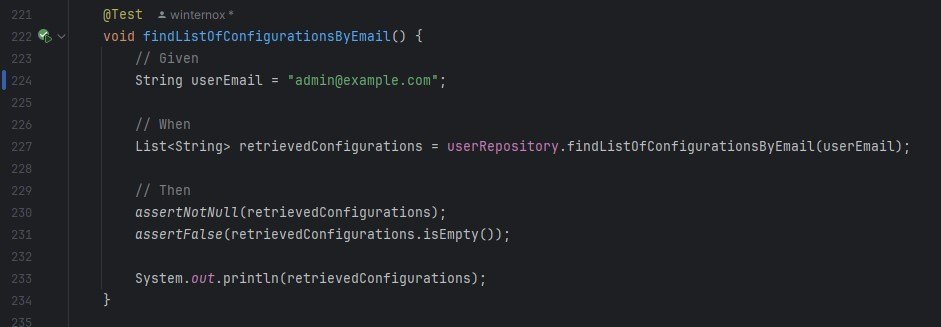
\includegraphics[width=0.8\textwidth]{images/5_testing/userdao-test}
    \caption{Testing the method of findListOfConfigurationsByEmail() in UserDAO class}
    \label{fig:u_dao_test}
\end{figure}

\begin{figure}[ht!]
    \centering
    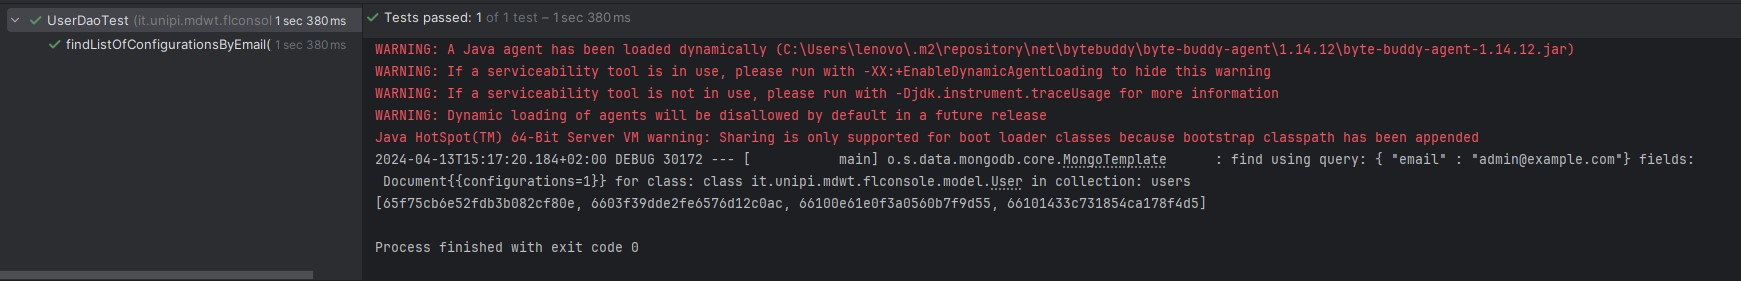
\includegraphics[width=0.8\textwidth]{images/5_testing/userdao-test-result}
    \caption{Testing result for the method of findListOfConfigurationsByEmail() in UserDAO class}
    \label{fig:u_dao_test_result}
\end{figure}

With this JUnit test method, the findListOfConfigurationsByEmail() method of the UserDAO class is tested. The test is performed by finding all the related configuration that are belong to the user with that email.
The test is successful and the expected result is returned as a list of configurations.

\newpage
\subsubsection{ExperimentDAO}
Experiment DAO is another important class of the project which is responsible for interacting with the database to handle data related with experiments. JUnit tests are created to ensure that the experiment related functions are
working as expected and the requirements are fulfilled. The tests are including creating new experiment, updating existing experiment, deleting existing experiment, finding experiment by some criterias. Below it can be seen an example test method for update an experiment.

\begin{figure}[ht!]
    \centering
    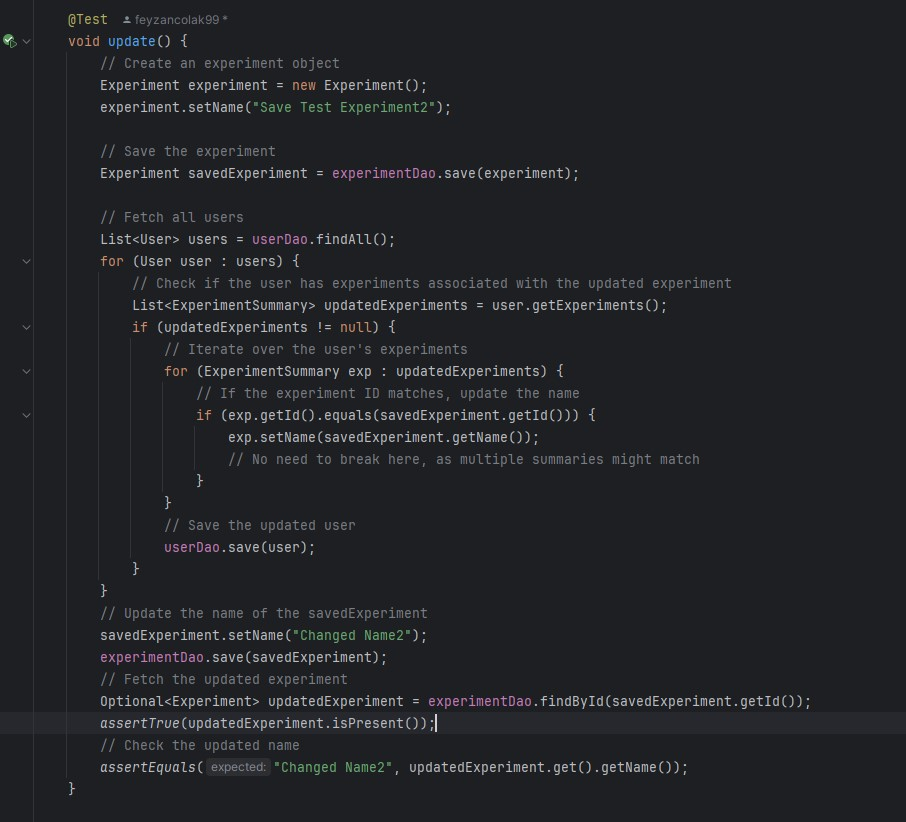
\includegraphics[width=0.8\textwidth]{images/5_testing/experimentdao-test}
    \caption{Testing the method of update() in ExperimentDAO class}
    \label{fig:e_dao_test}
\end{figure}

\newpage
\subsubsection{ConfigurationDAO}

Test class for Configuration DAO is another example of JUnit test that is performed on the project. The Configuration DAO class is responsible for interacting with the database to handle storage and retrival of the system experiment configuration.
Implementing JUnit for this class guarantees that system operates the data in an intended way for configuration class. Below there is an example test and test result for saveAndRetrieve() method of Configuration DAO class. The test is performed by
saving a configuration and then retrieving it from the database. The test is successful and the expected result is returned.

\begin{figure}[ht!]
    \centering
    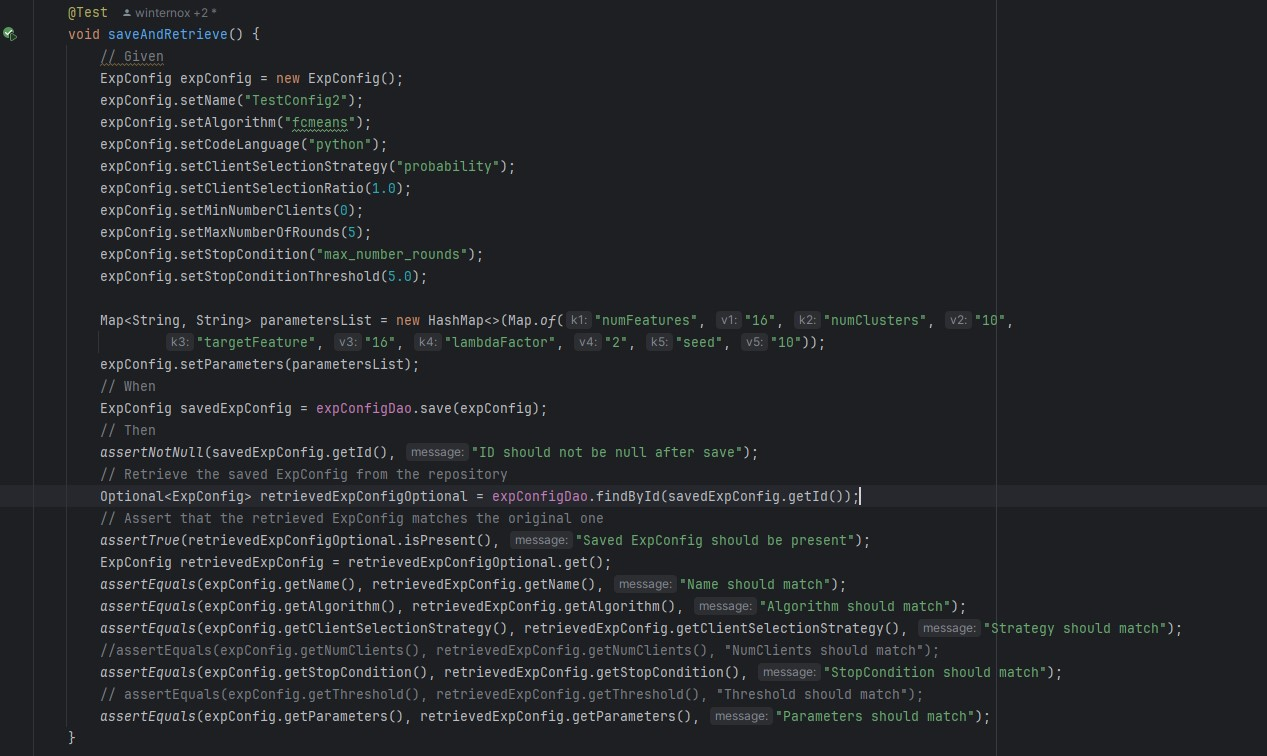
\includegraphics[width=0.8\textwidth]{images/5_testing/expconfigdao-test}
    \caption{Testing the method of saveAndRetrieve() in Configuration DAO class}
    \label{fig:c_dao_test}
\end{figure}

\begin{figure}[ht!]
    \centering
    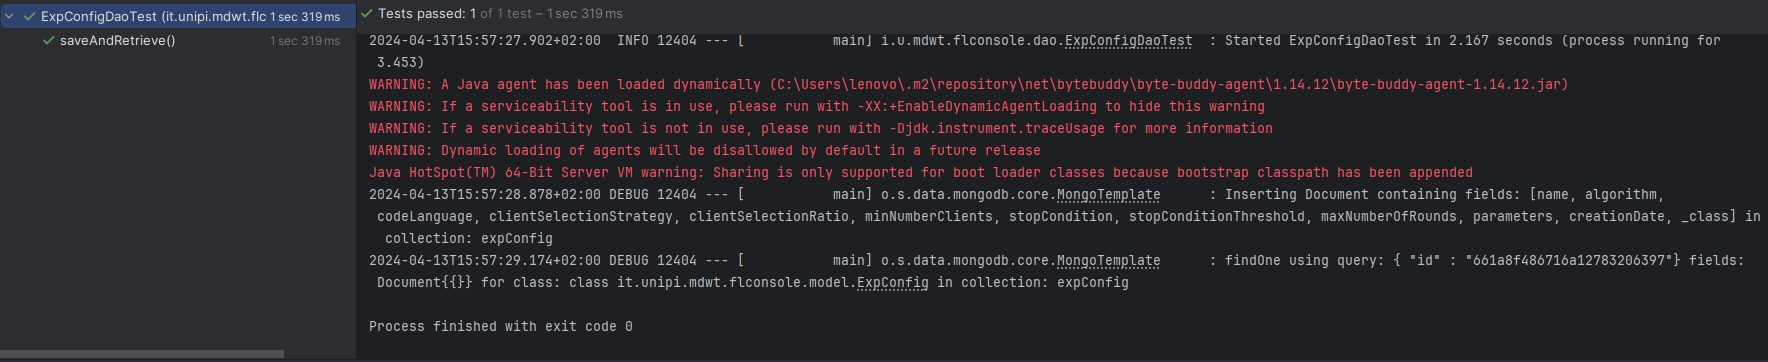
\includegraphics[width=0.8\textwidth]{images/5_testing/expconfigdao-test-result}
    \caption{Testing result for the method of saveAndRetrieve() in Configuration DAO class}
    \label{fig:c_dao_test_result}
\end{figure}


\newpage
\section{Functional Testing}

%The functional testing performed on the project is described in this section.
Functional testing, also known as black-box testing is applied to the project to evaluate the system behaviour that needs to fulfill functional requirements.
Functional testing helps to ensure that user expectations are provided in a right way. The functional testing is performed by creating test cases for the system.\\

Test cases are identified according to the functional requirements. It shows how the system should behave in different scenarios that are both normal and anormal.
Those test cases are including user authentication, creating new configuration, creating new experiment, deleting experiment, finding experiment, finding configuration, deleting configuration, etc.
Below there is a table that shows some examples of the test cases that are created for the project. As a result of the test cases, it can be said that the Federated Learning Web Console provides all the
necessary functionalities and meets user expectations.

\subsection{Test Cases}

%\begin{table}[ht!]
%    \centering
%    \caption{Test case}
%    \begin{tabularx}{\textwidth}{|Sl|S{X}|S{X}|S{X}|S{X}|S{X}|}
%        \hline
%        \textbf{Id} & \textbf{Description} & \textbf{Input} & \textbf{E. Output} & \textbf{Output} & \textbf{Outcome} \\ \hline
%        U\_T\_01    & Lorem Ipsum          & Lorem Ipsum    & Lorem Ipsum         & Lorem Ipsum     & Lorem Ipsum      \\ \hline
%        U\_T\_02    & Lorem Ipsum          & Lorem Ipsum    & Lorem Ipsum         & Lorem Ipsum     & Lorem Ipsum      \\ \hline
%        U\_T\_03    & Lorem Ipsum          & Lorem Ipsum    & Lorem Ipsum         & Lorem Ipsum     & Lorem Ipsum      \\ \hline
%        U\_T\_04    & Lorem Ipsum          & Lorem Ipsum    & Lorem Ipsum         & Lorem Ipsum     & Lorem Ipsum      \\ \hline
%        U\_T\_05    & Lorem Ipsum          & Lorem Ipsum    & Lorem Ipsum         & Lorem Ipsum     & Lorem Ipsum      \\ \hline
%    \end{tabularx}
%\end{table}


\begin{table}[ht!]
    \centering
    \caption{Admin Test case}
    \begin{tabularx}{\textwidth}{|c|>{\RaggedRight}p{2.2cm}|>{\RaggedRight}X|>{\RaggedRight}p{2.7cm}|>{\RaggedRight}p{1.98cm}|>{\RaggedRight}p{1.5cm}|}
        \hline
        \textbf{Id} & \textbf{Description} & \textbf{Input} & \textbf{Expected Output} & \textbf{Output} & \textbf{Outcome} \\
        \hline
        \multirow{2}{*}{A\_T\_01} & \multirow{2}{2.2cm}{Admin Login} & \multirow{2}{\linewidth}{Email: admin@example.com \\ Password: Adm1nP@ss (valid credentials)} & Login Successfully  & Redirected to admin dashboard & Passed \\
        & & & & & \\
        \hline
        \multirow{2}{*}{A\_T\_02} & \multirow{2}{2.2cm}{Admin Login 2} & Email: invalid@example.com & \multirow{2}{\linewidth}{Error message displayed} & Unable to login & Passed \\
        & & Password: invalid (invalid credentials) & & & \\
        \hline
        A\_T\_03 & Creating New Configuration & Adding all necessary values to the new FL configuration form & Configuration Created successfully & Configuration Created successfully & Passed \\
        \hline
        A\_T\_04 & Creating New Configuration 2 & Entering all values except stop condition & Error of missing value message displayed & Configuration is not created & Passed \\
        \hline
        A\_T\_05 & Creating New Experiment & Name is written and FL configuration is selected & Experiment Created successfully & Experiment Created successfully & Passed \\
        \hline
        A\_T\_06 & Starting an Experiment & Press Start Experiment button & Experiment starts & Experiment starts & Passed \\
        \hline
        \multirow{2}{*}{A\_T\_07} & \multirow{2}{2.2cm}{Search Configuration by name} & Write name with existing configuration name & \multirow{2}{\linewidth}{Show the list of the configuration with that name} & List of configurations with that name  & Passed \\
        \hline
        \multirow{2}{*}{A\_T\_08} & \multirow{2}{2.2cm}{Search experiment by name} & Write name with existing experiment name & \multirow{2}{\linewidth}{Show the list of the experiments with that name} & List of experiments with that name  & Passed \\
        \hline
    \end{tabularx}
\end{table}


\begin{table}[ht!]
    \centering
    \caption{User Test case}
    \begin{tabularx}{\textwidth}{|c|>{\RaggedRight}p{2.2cm}|>{\RaggedRight}X|>{\RaggedRight}p{2.7cm}|>{\RaggedRight}p{1.98cm}|>{\RaggedRight}p{1.5cm}|}
        \hline
        \textbf{Id} & \textbf{Description} & \textbf{Input} & \textbf{Expected Output} & \textbf{Output} & \textbf{Outcome} \\
        \hline
        \multirow{2}{*}{U\_T\_01} & \multirow{2}{2.2cm}{User Login} & \multirow{2}{\linewidth}{Email: firstTest@example.com \\ Password: P@ssw0rd (valid credentials)} & Login Successfully  & Redirected to user dashboard & Passed \\
        & & & & & \\
        \hline
        \multirow{2}{*}{U\_T\_02} & \multirow{2}{2.2cm}{User Login 2} & Email: wrong@example.com & \multirow{2}{\linewidth}{Error message displayed} & Unable to login & Passed \\
        & & Password: invalid (invalid credentials) & & & \\
        \hline
        \multirow{2}{*}{U\_T\_03} & \multirow{2}{2.2cm}{User Signup} & Email: new@example.com & Sign up successfully & Redirected to user dashboard & Passed \\
        & & Password: P@ssw0rd (valid input) & & & \\
        \hline
        \multirow{2}{*}{U\_T\_04} & \multirow{2}{2.2cm}{User Signup 2} & Email: new@example.com & \multirow{2}{\linewidth}{Error message displayed} & Unable to Signup & Passed \\
        & & Password: invalid (invalid password) & & & \\
        \hline
        \multirow{2}{*}{U\_T\_05} & \multirow{2}{2.2cm}{Search Configuration by name} & Write name with existing configuration name & \multirow{2}{\linewidth}{Show the list of the configuration with that name} & List of configurations with that name  & Passed \\
        \hline
        \multirow{2}{*}{U\_T\_06} & \multirow{2}{2.2cm}{Search experiment by name} & Write name with existing experiment name & \multirow{2}{\linewidth}{Show the list of the experiments with that name} & List of experiments with that name  & Passed \\
        \hline
    \end{tabularx}
\end{table}





\chapter{Conclusion}
%In this chapter, we summarize the key points of the document and discuss possible future directions for the project.


The project has delivered a robust web console for initiating federated learning experiments 
concurrently across remote environments. Leveraging Java Spring Boot with MVC pattern, 
WebSocket technology, and MongoDB as the backend database, a dynamic platform for real-time 
analytics and seamless communication between frontend and backend systems has been created.
\\
The implementation choices have proven effective, facilitating efficient communication and 
coordination between disparate components. By utilizing JInterface as a middleware to interface 
with the infrastructure managing federated learning experiments, seamless integration and 
enhanced interoperability have been achieved.
\\
Moreover, the design approach enables scalability and extensibility, laying the groundwork 
for future enhancements and expansions. The flexibility of the web console architecture allows 
for the incorporation of new experiment algorithms and the refinement of message structures to 
further optimize performance and functionality.
\\
Overall, the implementation demonstrates a well-thought-out approach that effectively meets 
the project's objectives. The successful deployment of the web console signifies not only the 
strength of the implementation choices but also the potential for continued innovation and 
growth in the realm of federated learning experimentation.


\end{document}